
\DIFdelbegin %DIFDELCMD < 

%DIFDELCMD < %%%
\DIFdelend The field of computational neutronics, computationally solving the Boltzmann Transport equation applied to neutrons (transport equation), is generally concerned with modeling neutrons in a nuclear system. These systems include nuclear reactors or shielding problems where there exists a fixed source of neutrons. The materials used in these systems have a variety of properties, including how they effect the energy of the neutron. Many materials that are commonly used in nuclear applications, particularly those containing hydrogen, exhibit a property known as upscattering, where lower energy neutrons are ``bounced" to higher energies. The details of scattering can dramatically impact which numerical methods to choose, particularly when solving the transport equation deterministically. 

\DIFdelbegin \DIFdel{Hydrogen based materials, such as graphite or heavy water, are often used as moderators in nuclear reactors. These problems, with upscattering and little leakage or absorption, are traditionally very computationally expensive ~\mbox{%DIFAUXCMD
\cite{morel-upscat}}\hspace{0pt}%DIFAUXCMD
. A significant cause of the large computational cost comes from the number of iterations needed to converge the problem.
}\DIFdelend %DIF >  This comes a bit too soon. You need to tell us you're solving the transport equation, that you're doing that deterministically, and that energy groups are a thing. Having this in the first paragraph is before we're ready for it. 
%DIF > Mathematically, a scattering matrix representing the scattering cross sections from group $\rg$ to $\rg'$ with the highest energy in group 1 and the lowest in group $G$ would be lower triangular if there is no upscattering. The entries $[\rg, \rg'\geq \rg]$ account for downscattering. A triangular matrix has nice computational properties that make the solving of the problem easier. However, when upscattering is present, the triangularity of the matrix is broken and other solution techniques must be employed. The most commonly used method in neutron transport calculations for problems with upscattering is known as the Gauss-Seidel Method. 
%DIF >  This whole paragraph should go somewhere else. It's also confusing and not quite right. 
\DIFaddbegin 

%DIF >  Instead, you might want to add a paragraph about impact and more broadly motivating this work. 

\DIFadd{In this work, we explore methods for speeding up nonlinear diffusion acceleration (NDA) in the presence of upscattering. NDA is also known as coarse-mesh finite difference and is a well-known technique applied to accelerate the scattering convergence in neutronics calculations. In multigroup neutronics problems, NDA is effective in conjunction with Gauss Seidel (GS) iteration in energy if there is little upscattering. However, when upscattering has a significant impact, which is common with thermal systems, the efficiency of GS-NDA degrades as extra iterations are required for convergence in energy \mbox{%DIFAUXCMD
\cite{park-nda}}\hspace{0pt}%DIFAUXCMD
.
}

\DIFadd{To remedy the issue in GS with upscattering, an energy two-grid (TG) acceleration scheme was first developed to approximate iteration error by solving a one-group diffusion-like equation with artificial material properties generated by using the scattering eigen-spectrum \mbox{%DIFAUXCMD
\cite{morel-upscat}}\hspace{0pt}%DIFAUXCMD
. Later, a transport TG (TTG) method was developed that approximates the energy error using a consistent }\sn\DIFadd{\ solver in multi-D \mbox{%DIFAUXCMD
\cite{evans-upscat}}\hspace{0pt}%DIFAUXCMD
. }[\DIFadd{need a statement here about why these either don't work with NDA or are insufficient st we need a new method}]\DIFadd{. Inspired by the previous studies, we derive a TG scheme for the NDA equation with GS iteration.
}

%DIF >  you need to flip the order of the TE section and previous work. Previous work mostly doesn't make any sense without seeing the TE and how it's discretized. The opening section barely makes sense. 

\section{\DIFadd{Previous Work}}
%DIF >  we definitely don't have enough information to understand this paragraph, even after the TE section. Please rewrite. 
\DIFadd{To accelerate the convergence of source iteration, a method that converges the flux inside of a given enegy group, Nonlinear Diffusion Acceleration was developed \mbox{%DIFAUXCMD
\cite{Knoll2011} }\hspace{0pt}%DIFAUXCMD
\mbox{%DIFAUXCMD
\cite{park-nda}}\hspace{0pt}%DIFAUXCMD
. 
%DIF >  Not sure if this is the right way to do it, but you haven't told us what SI is. 
NDA pairs a lower order equation with a higher order, drift diffusion equation. 
%DIF >  we also don't know what a drift diffusion equation is. 
As the higher order equation is not conservative, the method is formally inconsistent: the scalar flux and current may not be equal upon convergence,
%DIF >   equal to one another? Should they be? That doesn't make any sense to me. Or, the scalar flux and current in the higher order isn't equal to NDA? Please clarify.
%DIF >  Also, make sure to tell us what the scalar flux and current are.
although they are equal in the limit as the spatial mesh is refined. However, second order accuracy
%DIF >  which thing has second order accuracy? This also came out of nowhere
 can still be maintained with the high-order equation generally giving a more accurate shape and the conservative low-order equation giving a more accurate magnitude.
 %DIF >  you never told us the low order equation is conservative.  
 The combination of the two equations has been found to be more accurate than either equation alone \mbox{%DIFAUXCMD
\cite{morel-holo}}\hspace{0pt}%DIFAUXCMD
.
 }

\DIFadd{Since its development, NDA has been tried with a variety of higher order equations, \mbox{%DIFAUXCMD
\cite{morel-holo}}\hspace{0pt}%DIFAUXCMD
\mbox{%DIFAUXCMD
\cite{Wang2013} }\hspace{0pt}%DIFAUXCMD
as well as spatial discretizations \mbox{%DIFAUXCMD
\cite{morel-holo}}\hspace{0pt}%DIFAUXCMD
\mbox{%DIFAUXCMD
\cite{Schunert2017}}\hspace{0pt}%DIFAUXCMD
. In this work, we explore NDA with the Self-Adjoint Angular Flux Equation (SAAF) and a continuous finite element discretization.
}

%DIF >  the following paragraph is useful context. Needs to come earlier. 
\DIFaddend The steady-state transport equation is dependent on space, angle, and energy. It is often solved via a series of nested iterations. The various iteration methods and how they are used with each other are described in detail in Ch. \ref{sec:iterative}. \DIFdelbegin \DIFdel{In this work we target two layers of iteration, the ``within-group" and the "multi-group" iterations, attempting to reduce the total number of iterations needed and thus the run time. The first method we use, }\DIFdelend \DIFaddbegin \DIFadd{The }\DIFaddend Nonlinear Diffusion Acceleration \DIFdelbegin \DIFdel{(NDA), }\DIFdelend happens in the \DIFdelbegin \DIFdel{within-group, or source , }\DIFdelend \DIFaddbegin \DIFadd{source }\DIFaddend iteration, where angle and energy are fixed. \DIFdelbegin \DIFdel{The second method, which to our knowledge has never been applied to NDA, targets the multigroup solver, Gauss-Seidel. Gauss-Seidel is one of }\DIFdelend \DIFaddbegin \DIFadd{When energy is discretized into more than one energy group, an outer layer of iteration is introduced. One of }\DIFaddend the most commonly-used methods for iterating over energy groups \DIFdelbegin \DIFdel{. It }\DIFdelend \DIFaddbegin \DIFadd{is known as Gauss Seidel. Gauss Siedel }\DIFaddend is guaranteed to converge; however, in problems with significant upscattering, the time it takes to reach convergence can become arbitrarily slow\DIFdelbegin \DIFdel{\mbox{%DIFAUXCMD
\cite{evans-upscat}}\hspace{0pt}%DIFAUXCMD
, which makes it a good candidate for acceleration}\DIFdelend . 
%DIF >  probably need a citation for that claim.

\DIFdelbegin \DIFdel{To accelerate the Gauss-Seidel convergence with upscattering, an energy two-grid (TG) acceleration scheme was first developed to approximate iteration error by solving a }\DIFdelend \DIFaddbegin \DIFadd{A number of techniques to accelerate Gauss Seidel convergence have been developed \mbox{%DIFAUXCMD
\cite{morel-upscat} }\hspace{0pt}%DIFAUXCMD
\mbox{%DIFAUXCMD
\cite{evans-upscat}}\hspace{0pt}%DIFAUXCMD
, although to our knowledge none have yet been paired with NDA. The primary techniques used in commercial transport software rely on a rebalance scheme and coarse-mesh finite-difference diffusion.
%DIF >  I'm not sure we can understand what that means either. 
Although these methods are widely used and successful for acceleration, they are very sensitive to the coarse mesh size. Rebalancing with too fine a mesh may be divergent, and an overly coarse mesh degrades performance \mbox{%DIFAUXCMD
\cite{evans-upscat}}\hspace{0pt}%DIFAUXCMD
.
}

\DIFadd{While for standard problems, the proper mesh size is generally well understood;
%DIF >  I don't know what is a standard problem; shielding isn't non-standard...???
 this is not the case for shielding problems. Adams and Morel developed an upscatter acceleration scheme known as the Two-Grid method. An estimation of the error at each Gauss Seidel iteration is calculated using a collapsed in energy, }\DIFaddend one-group \DIFdelbegin \DIFdel{diffusion-like equation with artificial material properties generated by using the scattering eigen-spectrum \mbox{%DIFAUXCMD
\cite{morel-upscat}}\hspace{0pt}%DIFAUXCMD
. Later, a transport TG (TTG) methodwas developed that approximates the energy error using a consistent }%DIFDELCMD < \sn%%%
\DIFdel{\ solver in multi-D \mbox{%DIFAUXCMD
\cite{evans-upscat}}\hspace{0pt}%DIFAUXCMD
. Both of these were developed for use with traditional source iteration, and to our knowledge have not yet been extended for use with NDA. Inspired by the previous studies, we derive a TG scheme for the NDA equation with Gauss-Seidel iteration. }\DIFdelend \DIFaddbegin \DIFadd{diffusion equation and energy eigenvector of the Gauss Seidel iteration matrix. These
 %DIF >  I don't know what "these" means here
  make up the correction term to the scalar flux at each group, which is applied at each iteration. In one dimensional calculations, Adams and Morel have demonstrated their method to be very efficient for thermal upscattering problems \mbox{%DIFAUXCMD
\cite{morel-upscat}}\hspace{0pt}%DIFAUXCMD
.
}\DIFaddend 


%DIF >  It might be helpful to use a few sentences about what methods you use to frame what you tell us below. I think that will help us to follow along for all of what comes next. E.g. "This work uses Nonlinear Diffusion Acceleration. NDA reformulates the transport equation as a correction to the diffusion equation and uses a two step process to solve it." and then tell us about the stuff you're going to tell us.
%DIF >  Also, I'm not clear why we need the k-eigenvalue form. It seems like a distraction. 
\section{The Boltzmann Transport Equation}
The angular neutron flux of a reactor, $\psi$ can be found by solving the steady state Boltzmann Transport equation,
%DIF > 
\DIFaddbegin \begin{equation}
\DIFadd{\begin{split}
 [\hat{\Omega} \cdot \nabla + &\Sigma(\vec{r}, E)]\psi(\vec{r}, \hat{\Omega}, E) = \chi(E) \int_0^\infty dE' \nu \Sigma_{f}(\vec{r}, E') \int_{4\pi} d\hat{\Omega}'\psi(\vec{r}, \hat{\Omega}', E') \\   &+ \int_0^\infty dE' \int_{4\pi} d\hat{\Omega}' \Sigma_s(\vec{r}, E' \rightarrow E, \hat{\Omega}' \cdot \hat{\Omega})\psi(\vec{r}, \hat{\Omega}', E') + Q(\vec{r}, \hat{\Omega}, E)   \:,
\end{split}
\label{eq:transport}
}\end{equation}
\DIFaddend 


\DIFdelbegin \begin{displaymath}
\DIFdel{\begin{split}
  [\hat{\Omega} \cdot \nabla + &\Sigma_t(\vec{r}, E)]\psi(\vec{r}, \hat{\Omega}, E) = \frac{\chi(E)}{4\pi} \int_0^\infty dE' \nu \Sigma_{f}(\vec{r}, E') \int_{4\pi} d\hat{\Omega}'\psi(\vec{r}, \hat{\Omega}', E') \\   &+ \int_0^\infty dE' \int_{4\pi} d\hat{\Omega}' \Sigma_s(\vec{r}, E' \rightarrow E, \hat{\Omega}' \cdot \hat{\Omega})\psi(\vec{r}, \hat{\Omega}', E') + Q(\vec{r}, \hat{\Omega}, E)   \:,
\end{split}
%DIFDELCMD < \label{eq:transport}%%%
}\end{displaymath}
%DIFAUXCMD
%DIFDELCMD < 

%DIFDELCMD < %%%
\DIFdelend where $\hat{\Omega}$ represents the angle; $\vec{r}$, the position vector; $E$, the energy; \DIFdelbegin \DIFdel{$\Sigma_t$}\DIFdelend \DIFaddbegin \DIFadd{$\Sigma$}\DIFaddend , the total macroscopic cross-section; $\Sigma_f$, the macroscopic fission cross-section; $\Sigma_s$, the macroscopic scattering cross section; $\chi$, the \DIFaddbegin \DIFadd{fission }\DIFaddend energy distribution; \DIFdelbegin \DIFdel{and }\DIFdelend $\nu$, the average number of neutrons per fission; and $Q$, an external source. 

In this work, we apply an incident boundary condition, where for $\hat{n} \cdot \hat{\Omega} < 0$, with $\hat{n}$ being the outward normal on the boundary $\partial \mathcal{D}$,
\begin{equation}
    \psi(\vec{r}, \hat{\Omega}, E) = \psi^{inc}(\vec{r}, \hat{\Omega}, E), \hspace{5mm} \vec{r} \in \partial \mathcal{D}\:,
\end{equation}
though other boundary conditions such as reflecting, periodic, and vacuum are valid.

\subsection{\DIFdelbegin \DIFdel{Fixed Source Form }\DIFdelend \DIFaddbegin \DIFadd{Forms }\DIFaddend of the Transport Equation}
There are are several forms of the transport equation that are of interest in the field of nuclear energy. 
\DIFdelbegin \DIFdel{In this work, we present all methods in fixed-source form; however, they can all be easily extended to $k$-eigenvalue form for criticality calculations. 
}\DIFdelend 

\DIFaddbegin \subsubsection{\DIFadd{Fixed Source Form}}
\DIFaddend To write Eqn.~\eqref{eq:transport} in a fixed source form, we drop the fission term and retain the source, $Q$. If there is fission in the system, fission neutrons can be included in the source term. We use the same boundary conditions as above. 
%
\begin{equation}
\begin{split}
 [\hat{\Omega} \cdot \nabla + \Sigma(\vec{r}, E)]\psi(\vec{r}, \hat{\Omega}, E) &= \\ \int_0^\infty dE' &\int_{4\pi} d\hat{\Omega}' \Sigma_s(\vec{r}, E' \rightarrow E, \hat{\Omega}' \cdot \hat{\Omega})\psi(\vec{r}, \hat{\Omega}', E')  + Q(\vec{r}, \hat{\Omega}, E)
\end{split}
 \label{eq:transport_fixed_source}
\end{equation}

\DIFaddbegin \subsubsection{\DIFadd{$k$-Eigenvalue Form}}
\DIFadd{When fission is in a system, we are often interested in the multiplication behavior, which can be described by a parameter, $k$, the ratio of neutrons in two successive generations. If the chain reaction is self-sustaining and time-independent, the reactor is known as ``critical" and $k=1$. A $k>1$ gives an increasing population, termed supercritical, and $k<1$ gives a subcritical, decreasing population. We scale $\nu$ in Eq. }\eqref{eq:transport} \DIFadd{by $k$ to express the deviation from critical. This gives the following equation,
%DIF > 
}\begin{equation}
    \DIFadd{\label{eq:transport_eigenvalue}
    \begin{split}
        [\hat{\Omega} \cdot \nabla + \Sigma(\vec{r}, E)]\psi(\vec{r}, \hat{\Omega}, E) &= \frac{\chi(E)}{4\pi k} \int_0^\infty dE' \nu \Sigma_{f}(\vec{r}, E') \int_{4\pi} d\hat{\Omega}'\psi(\vec{r}, \hat{\Omega}', E') \\ &+ \int_0^\infty dE' \int_{4\pi} d\hat{\Omega}' \Sigma_s(\vec{r}, E' \rightarrow E, \hat{\Omega}' \cdot \hat{\Omega})\psi(\vec{r}, \hat{\Omega}', E') \ :,
    \end{split}
}\end{equation}
\DIFadd{where the $\frac{1}{4\pi}$ is added to represent that fission neutrons are born isotropically. We again using the same boundary conditions. 
}

\DIFadd{Eqn.~}\eqref{eq:transport_eigenvalue} \DIFadd{is an eigenvalue problem that, with some algebraic manipulation, can be written of in the form $A\psi = \frac{1}{k} F\psi$ and solved via standard eigenvalue solvers. 
}

\DIFadd{In this work, we present all methods in fixed-source form; however, they can all be easily extended to $k$-eigenvalue form for criticality calculations. 
}

\DIFaddend \section{Space-Angle Approximations of Interest}
There are many simplifications and approximations that can be made to facilitate the solution of the transport equation. In this work, we assume our scattering and fixed sources are isotropic, which gives the following form
%
\begin{equation}
\DIFdelbegin %DIFDELCMD < \begin{split}
%DIFDELCMD < 

%DIFDELCMD < [\hat{\Omega} \cdot \nabla + \Sigma_t(\vec{r}, E)]\psi(\vec{r}, \hat{\Omega}, E) &= \\  \int_0^\infty \frac{1}{4\pi} &\Sigma_s(\vec{r}, E' \rightarrow E)  dE' \int_{4\pi} d\hat{\Omega}'\psi(\vec{r}, \hat{\Omega}', E')  + \frac{1}{4\pi}Q.
%DIFDELCMD < 

%DIFDELCMD < \end{split}
%DIFDELCMD <  %%%
\DIFdelend \DIFaddbegin \begin{split}
 [\hat{\Omega} \cdot \nabla + \Sigma(\vec{r}, E)]\psi(\vec{r}, \hat{\Omega}, E) &= \\ \frac{1}{4\pi}  \int_0^\infty &\Sigma_s(\vec{r}, E' \rightarrow E)  dE' \int_{4\pi} d\hat{\Omega}'\psi(\vec{r}, \hat{\Omega}', E')  + \frac{1}{4\pi}Q \:.
\end{split}
 \DIFaddend \label{eq:transport_isotropic_scattering}
\end{equation}
%
This equation gives the angular flux. To find the scalar flux, $\phi$, which is often the quantity desired in practice at it is used to give the reactions rates needed for engineering solutions, we must integrate over all directions
\DIFaddbegin \begin{equation}
    \DIFadd{\phi(\vec{r}, E) = \int_{4\pi} \phi(\vec{r}, \hat{\Omega}, E) d \Omega \:.
}\end{equation}
\DIFaddend 

\DIFdelbegin \begin{displaymath}
  \DIFdel{\phi(\vec{r}, E) = \int_{4\pi} \phi(\vec{r}, \hat{\Omega}, E) d \hat{\Omega}\:.
}\end{displaymath}
%DIFAUXCMD
\DIFdelend \DIFaddbegin \subsection{\DIFadd{Self-Adjoint Angular Flux}}
\DIFadd{Discretizing the traditional transport equation, Eqn.~}\eqref{eq:transport_isotropic_scattering}\DIFadd{, in space, particularly using the finite element method, presents a number of challenges \mbox{%DIFAUXCMD
\cite{saaf}}\hspace{0pt}%DIFAUXCMD
. A finite element spatial discretization is generally favorable as it produces as symmetric positive-definite (SPD) linear system. SPD systems can be solved using a number of well-studied, robust solution techniques. In order to make use of these properties, we must rearrange the standard transport equation into a form that is more computationally friendly, a self-adjoint form \mbox{%DIFAUXCMD
\cite{saaf}}\hspace{0pt}%DIFAUXCMD
.
}\DIFaddend 

\DIFaddbegin \DIFadd{The monoenergetic version of the Self-Adjoint Angular Flux equation appropriate for $S_N$ calculations is 
%DIF >  you didn't tell us what an SN calculation is yet
}\begin{equation}
    \DIFadd{- \vec{\Omega} \cdot \nabla \frac{1}{\Sigma_t}\vec{\Omega} \cdot \nabla \psi + \Sigma_t \psi = \frac{1}{4\pi}[\Sigma_s\phi + Q - \vec{\Omega} \cdot \nabla \frac{(\Sigma_s\phi + Q)}{\Sigma_t}]\:.
    \label{eq:SAAF}
}\end{equation}
%DIF >  do you use the monoenergetic form? This section feels a little out of nowhere. Maybe an additional sentence or two telling us why you're telling us this out of every possible spatial discretization form. 


\DIFaddend \subsection{The Diffusion Equation}
To simplify even further, we employ a commonly-used approximation known as the diffusion equation. To derive the diffusion equation, we consider the neutron balance within an infinitesimal volume centered at a point, $r$. For simplicity of notation, we will present this derivation assuming all neutrons have the same energy. Under steady state conditions, neutron conservation requires
%
\begin{equation}
    \textit{neutrons leaking out} + \textit{neutrons absorbed} = \textit{source neutrons emitted}.
\end{equation}
We describe the neutrons leaking out as the rate of the current, \DIFdelbegin \DIFdel{$\vec{J} = \int_{4\pi} \vec{\Omega}\psi$ }\DIFdelend \DIFaddbegin \DIFadd{$J$}\DIFaddend , in all directions; the neutrons absorbed is the absorption cross section times the scalar flux, $\Sigma_a\phi$; and the source neutrons are represented by the source variable, $Q$. This gives the neutron continuity equation
%DIF >  I'd put in the equaiton for current so we know how it fits in to this whole thing.
\begin{equation}
    \DIFdelbegin %DIFDELCMD < 

%DIFDELCMD < %%%
\DIFdelend \nabla\cdot \vec{J}(\vec{r}) + \Sigma_a(\vec{r})\phi(\vec{r}) = Q(\vec{r})\:.
\DIFdelbegin %DIFDELCMD < 

%DIFDELCMD < %%%
\DIFdelend \end{equation}
Using Fick's Law, which relates the current to the flux, $\vec{J}(\vec{r}) = -D(\vec{r})\nabla\phi(\vec{r})$ where $D = 1/3\Sigma_t$, we get the diffusion approximation

\begin{equation}
\begin{split}
 - \nabla \cdot D(\vec{r})\nabla\phi(\vec{r}) &+ \Sigma_a \phi(\vec{r}) = Q(\vec{r})\:.
\end{split}
\label{eq:diffusion_fixed_source}
\end{equation}

The diffusion equation is much easier to solve than the transport equation because it is not dependent on angle. However, because of the assumptions made in the Fick's Law approximation, it is not valid near boundaries where material properties change dramatically, near localized sources, or in strongly absorbing media \cite{lewis-miller}.

\subsection{Nonlinear Diffusion Acceleration}
\DIFdelbegin %DIFDELCMD < 

%DIFDELCMD < %%%
\DIFdel{This work presents an acceleration to a method known as }\DIFdelend \DIFaddbegin \DIFadd{This work uses }\DIFaddend Nonlinear Diffusion Acceleration\DIFdelbegin \DIFdel{(NDA)}\DIFdelend . NDA reformulates the transport equation as a correction to the diffusion equation and uses a two step process to solve \DIFaddbegin \DIFadd{it}\DIFaddend . For reference, we repeat the derivation of the low-order NDA equation found in \cite{morel-holo} with small modifications \DIFdelbegin \DIFdel{. We assume }\DIFdelend \DIFaddbegin \DIFadd{assuming }\DIFaddend no fission source and vacuum boundary conditions. Consider the first order, one-group, fixed-source, steady-state $S_N$ transport equation with isotropic scattering
\DIFdelbegin \DIFdel{. 
}%DIFDELCMD < 

%DIFDELCMD <   %%%
\DIFdelend %DIF > 
  \begin{equation}
  \DIFdelbegin %DIFDELCMD < \hat{\Omega}%%%
\DIFdelend \DIFaddbegin \vec{\Omega}\DIFaddend \cdot \nabla \psi \left(\vec{r}\right)+ \Sigma_{\mm{t}}\left(\vec{r}\right)\psi = \frac{1}{4 \pi} \Sigma_{\mm{s}}\left(\vec{r}\right) \phi\left(\vec{r}\right) + \frac{1}{4 \pi} Q\:.
  \end{equation}
Integrate over all angles to obtain the zeroth moment equation
\begin{equation}
  \DIFdelbegin %DIFDELCMD < 

%DIFDELCMD <   %%%
\DIFdelend \nabla \cdot \vec{J} + \Sigma_a\phi  =  Q\DIFaddbegin \DIFadd{\:}\DIFaddend ,
  \label{eq:zeroth_moment_1g}
  \end{equation}
% where $\vec{J} = \int_{4\pi} \vec{\Omega}\psi$  (tell us this where you talk about current earlier)
Now consider the first moment equation
  \DIFdelbegin \DIFdel{:
  }\DIFdelend \begin{equation}
  \nabla \cdot \overset{\text{\scriptsize$\leftrightarrow$}}{P} + \Sigma_t J = 0 \DIFaddbegin \DIFadd{\:}\DIFaddend ,
  \end{equation}
where $\nabla \cdot \overset{\text{\scriptsize$\leftrightarrow\DIFdelbegin \DIFdel{$}}{P} =  \int_{4\pi} \hat{\Omega} \hat{\Omega} \cdot \nabla \psi$. It }\DIFdelend \DIFaddbegin \DIFadd{$}}{P} =  \int_{4\pi} \vec{\Omega} \vec{\Omega} \cdot \nabla \psi$. The first moment equation }\DIFaddend can be rewritten as
\DIFdelbegin \DIFdel{: 
}%DIFDELCMD < 

%DIFDELCMD <   %%%
\DIFdelend %DIF > 
  \begin{equation}
  J= -\frac{1}{\Sigma_t} \nabla \cdot \overset{\text{\scriptsize$\leftrightarrow$}}{P}\:. 
  \end{equation}
  By adding and subtracting the diffusion coefficient multiplied by the gradient of the scalar flux, the first moment equation takes the form of a correction to Fick's Law
  \begin{equation}
  J = -D \nabla \phi + D \nabla \phi - \frac{1}{\Sigma_t} \nabla \overset{\text{\scriptsize$\leftrightarrow$}}{P} \\
  \DIFdelbegin %DIFDELCMD < 

%DIFDELCMD <   %%%
\DIFdelend = -D \nabla \phi - \vec{\textbf{D}} \phi\DIFaddbegin \DIFadd{:}\DIFaddend ,
  \DIFdelbegin %DIFDELCMD < 

%DIFDELCMD <   %%%
\DIFdelend \label{eq:fick_corr_1g}
  \end{equation}
  where $\vec{\textbf{D}}$ is the drift vector
 \begin{equation}
  \vec{\textbf{D}} (\psi) = \DIFdelbegin \DIFdel{\frac{\int_{4\pi} [\frac{1}{\Sigma_t} \hat{\Omega} \hat{\Omega}\cdot \nabla \psi] - D \nabla \phi^{ho}}{\phi^{ho}}}\DIFdelend \DIFaddbegin \DIFadd{\frac{\int_{4\pi} [\frac{1}{\Sigma_t} \vec{\Omega} \vec{\Omega}\cdot \nabla \psi] - D \nabla \phi^{ho}}{\phi^{ho}}}\DIFaddend .
  \label{eq:drift_vector}
  \end{equation} 
\DIFdelbegin \DIFdel{Where $\psi^{ho} = \int_{4\pi} \psi(\hat{\Omega}, \vec{r}) d\hat{\Omega}$ }\DIFdelend \DIFaddbegin \DIFadd{Here, $\psi^{ho} = \int_{4\pi} \psi(\Omega, \vec{r}) d\Omega$ }\DIFaddend where $\psi$ is the solution of the higher order equation. \DIFdelbegin \DIFdel{Subsituting Eqn.}\DIFdelend \DIFaddbegin \DIFadd{Plugging Eqn.~}\DIFaddend \eqref{eq:fick_corr_1g} into \DIFaddbegin \DIFadd{Eqn.~}\DIFaddend \eqref{eq:zeroth_moment_1g}\DIFaddbegin \DIFadd{, }\DIFaddend we have the following NDA equation
  \DIFdelbegin \DIFdel{:
}%DIFDELCMD < 

%DIFDELCMD <   %%%
\DIFdelend \begin{equation}
  \nabla\cdot(-D \nabla \phi - \vec{\bf D} \phi) + \Sigma_a \phi = Q \:. \label{eq:NDA_1g}
  \end{equation}

Because NDA uses the solution from a higher-order calculation to find the the drift vector, it will not give an exact correction. While NDA maintains much of the accuracy of the higher-order equation when compared to diffusion, the two are not exactly equal. 


\subsection{\DIFdelbegin \DIFdel{Self-Adjoint Angular Flux}\DIFdelend \DIFaddbegin \DIFadd{Coupling NDA and SAAF}\DIFaddend }
\DIFdelbegin \DIFdel{NDA requires the use of a higher order equation. }\DIFdelend In this work, we use \DIFaddbegin \DIFadd{SAAF as }\DIFaddend the \DIFdelbegin \DIFdel{Self-Adjoint Angular Flux Form (SAAF ) \mbox{%DIFAUXCMD
\cite{SAAF}}\hspace{0pt}%DIFAUXCMD
. Discretizing the traditional transport equation Eqn.~}%DIFDELCMD < \eqref{eq:transport_isotropic_scattering} %%%
\DIFdel{in space, particularly using the finite element method presents a number of challenges \mbox{%DIFAUXCMD
\cite{saaf}}\hspace{0pt}%DIFAUXCMD
. A finite element spatial discretization is generally favorable as it produces as symmetric positive-definite (SPD) linear system. SPD systems can be solved using a number of well-studied, robust solution techniques \mbox{%DIFAUXCMD
\cite{Shewchuck1994}}\hspace{0pt}%DIFAUXCMD
. In order to make use of these properties, we must rearrange the standard transport equation into a form that is more computationally friendly.
}%DIFDELCMD < 

%DIFDELCMD < %%%
\DIFdel{The Self-Adjoint Angular Flux equation is given as
}%DIFDELCMD < 

%DIFDELCMD < %%%
\begin{displaymath}
    \DIFdel{- \vec{\Omega} \cdot \nabla \frac{1}{\Sigma_t}\vec{\Omega} \cdot \nabla \psi + \Sigma_t \psi = \frac{1}{4\pi}[\Sigma_s\phi + Q - \vec{\Omega} \cdot \nabla \frac{(\Sigma_s\phi + Q)}{\Sigma_t}]\:.
    %DIFDELCMD < \label{eq:SAAF}%%%
}\end{displaymath}
%DIFAUXCMD
%DIFDELCMD < 

%DIFDELCMD < %%%
\subsection{\DIFdel{Coupling NDA and SAAF}}
%DIFAUXCMD
\addtocounter{subsection}{-1}%DIFAUXCMD
\DIFdel{NDA and SAAF work together as an acceleration to }\DIFdelend \DIFaddbegin \DIFadd{higher order equation and NDA to accelerate the convergence of source iteration. 
%DIF >  You probably need to tell us what source iteration is more than I wrote above.
The implementation of }\DIFaddend the \DIFdelbegin \DIFdel{source iteration process. 
Source iteration is a method by which the scalar flux on the right hand side of Eqn. }%DIFDELCMD < \eqref{eq:transport_fixed_source} %%%
\DIFdel{is fixed, so that the equation may be solved with a linear solver. At each iteration, the result of $\phi$ at the previous iteration is used as the guess, until the solutions converge. NDA accelerates source iteration by using a higher order equation to create a correction to the diffusion equation. In this work, we use SAAF as the higher order equation. Below we outline how they work together, using $l$ as the iteration index.
}\DIFdelend \DIFaddbegin \DIFadd{algorithm is outlined below:
}\DIFaddend 

\begin{enumerate}
    \item Intitialize system, by setting $\vec{\textbf{D}}$ to 0 and solving Eqn.~\eqref{eq:NDA_1g} to get $\phi^0$ 
    \item Loop Until Convergence:
        \begin{enumerate}
            \item Solve Eqn.~\eqref{eq:SAAF} for $\psi^l$ using $\phi^{l-1}$ on RHS.
            \item Calculate drift vector, Eqn.~\eqref{eq:drift_vector}, using $\psi^l$
            \item Solve Eqn.~\eqref{eq:NDA_1g} for $\phi^l$
            \item Check $\phi^{l-1}, \phi^l$ for convergence
        \end{enumerate}
    \item Return $\phi$
\end{enumerate}

\DIFdelbegin \DIFdel{We }\DIFdelend \DIFaddbegin \DIFadd{While we }\DIFaddend are able to replicate the results of \cite{Wang2013}, showing a significant reduction in the number of source iterations necessary when using NDA with SAAF as compared to SAAF alone\DIFdelbegin \DIFdel{. However}\DIFdelend , NDA only \DIFdelbegin \DIFdel{accelerates }\DIFdelend \DIFaddbegin \DIFadd{acclerates }\DIFaddend one layer of iteration. The presence of upscattering introduces another layer of iteration: Gauss-Seidel iteration in energy. \DIFdelbegin \DIFdel{The number of Gauss-Seidel Iterations can become prohibitively large when there is significant upscattering. }\DIFdelend In the following section we derive an acceleration scheme \DIFdelbegin \DIFdel{to lessen the number of Gauss-Seidel iterations}\DIFdelend \DIFaddbegin \DIFadd{for the outer layer of iteration}\DIFaddend .


\section{Methods of Discretization}
The angular flux, $\psi$, is a function of space, angle, and energy. In the solution process, each dimension is discretized. There are several choices that have to be made regarding discretization. In this work, we endeavor to show equation forms that are discretization agnostic as well as showing formulations unique to the particular discretization methods we chose to implement. 

\subsection{Angular Discretization}


%DIF >  all angles are handled with this, not just one side.
%DIF > We assume the sources are isotropic and therefore do not perform any additional expansion; however, the scattering and fixed sources can be expanded via Spherical Harmonics and the methods will still hold. 
%DIF >  this sentence doesn't make mch sense unless you already know about expansion. I think you don't need to comment on that here. 
%DIF > 
\begin{figure}[H]
    \centering
    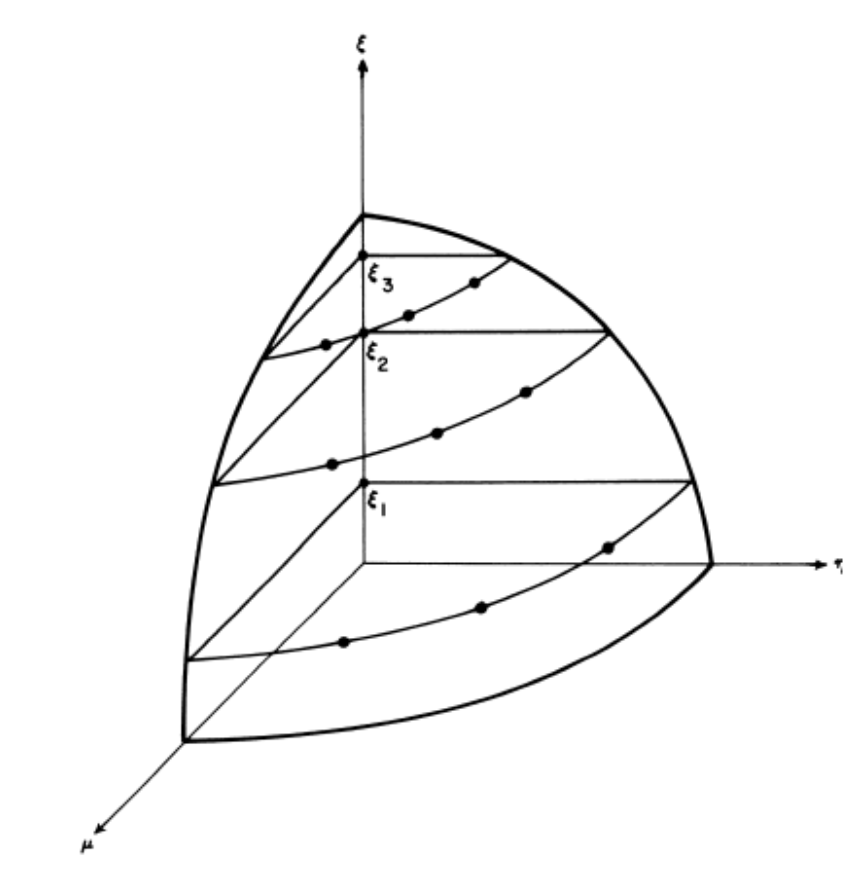
\includegraphics[width=.5\textwidth]{fig/SNPoints.png}
    \caption{Equally-Weighted Gauss-Chebyshev Quadrature Points \cite{Lathrop1965}}
    \label{fig:SN}
\end{figure}
%
Angular discretization of Eqn.~\eqref{eq:transport} is handled via the discrete ordinates ($S_N$) method, a finite-element collocation method \cite{Lathrop1965}. The $S_N$ method uses a quadrature rule, evaluating the equation at number of discrete angles or ``ordinates" and uses corresponding weights to perform a sum that results in integration over the unit sphere. 
For a set of $N$ ordinates with weights $w_n$, a function $f$ integrated over angle as
%
\begin{equation}
\DIFdelbegin %DIFDELCMD < 

%DIFDELCMD < %%%
\DIFdelend \int \DIFdelbegin %DIFDELCMD < \hat{\Omega} %%%
\DIFdelend f(\DIFdelbegin %DIFDELCMD < \hat{\Omega}%%%
\DIFdelend \DIFaddbegin \DIFadd{\Omega}\DIFaddend ) d\DIFdelbegin %DIFDELCMD < \hat{\Omega} %%%
\DIFdelend \DIFaddbegin \DIFadd{\Omega }\DIFaddend = \sum\limits\DIFdelbegin \DIFdel{_{\mrm=1}^{M} }\DIFdelend \DIFaddbegin \DIFadd{_{n=1}^{N} }\DIFaddend w\DIFdelbegin \DIFdel{_\mrm }\DIFdelend \DIFaddbegin \DIFadd{_n }\DIFaddend f\DIFdelbegin \DIFdel{_\mrm}\DIFdelend \DIFaddbegin \DIFadd{_n \:}\DIFaddend .  
\DIFdelbegin %DIFDELCMD < 

%DIFDELCMD < %%%
\DIFdelend \end{equation}
\DIFdelbegin %DIFDELCMD < 

%DIFDELCMD < %%%
\DIFdelend %DIF > To choose quadrature points, an octant of the unit sphere is discretized into several levels. At each level several nodes are chosen. 
%DIF >  that's not true generically for quadrature points.
We use a Gauss-Chebyshev angular quadrature set, which can be thought of as a product set, combining a one-dimensional Gaussian Quadrature along the polar angles and an equally-weighted Chebyshev quadrature along the azimuthal angles \cite{jarrel-thesis}. This can be seen in Figure~\ref{fig:SN}. 

The steady-state, one-group $S_N$ transport equation is given as follows,
\DIFdelbegin %DIFDELCMD < 

%DIFDELCMD <  %%%
\DIFdelend %DIF > 
 \begin{equation}
  \vec{\Omega}_n \cdot \nabla \psi_n \left(\vec{r}\right)+ \Sigma_{\mm{t}}\left(\vec{r}\right)\psi_n = \frac{1}{4 \pi} \Sigma_{\mm{s}}\left(\vec{r}\right) \phi\left(\vec{r}\right) + \frac{1}{4 \pi} Q\left(\vec{r}\right)\:,
  \label{eq:transport-angular}
 \end{equation}
where $n$ is the angular index and $\phi = \sum\limits_{n=1}^N \omega_n \psi_n$.
%DIF >  you don't have to switch to n, but it's the standard notation in the field and might confuse people. Hence S_N, not S_M. 

\subsection{Energy Discretization}
In our treatment of energy, we divide the full energy spectrum into several energy groups. By convention, the highest energy group is given the index, 1, with the index number going up until it reaches the lowest energy group, $G$. In expanding to multiple energy groups, we must take into account scattering from one group, $\rg'$ to another, $\rg$, denoted as $\rg' \rightarrow \rg $. 

The energy discretized, steady-state, transport equation is
%
 \begin{equation}
  \vec{\Omega} \cdot \nabla \psi_\rg \left(\vec{r}\right)+ \Sigma_{\mm{t}, \rg}\left(\vec{r}\right)\psi_\rg = \frac{1}{4 \pi} \sum\limits_{\rg'=1}^{G}\Sigma_{\mm{s}, \rg' \rightarrow \rg}\left(\vec{r}\right) \phi_{\rg'}\left(\vec{r}\right) + \frac{1}{4 \pi} Q_\rg\:.
  \label{eq:transport-energy}
 \end{equation}


\subsection{Spatial Discretization}
In this work, we choose to discretize in two dimensions, assuming uniformity in the third; however, all formulations could be extended to be truly 3D. Spatial discretization methods for the transport equation are usually performed using commonly-known differential equation discretization techniques such as the finite difference, finite volume, or finite element methods. In this work we, discretize using the finite element method on triangular elements (described in detail in Appendix \ref{sec:spatial}); however, TG-NDA can be used with any spatial discretization. We give the weak forms of NDA and SAAF. Their full derivations can be seen in Appendix \ref{sec:spatial}. 


\subsubsection{Weak Form of Multigroup NDA}

Given a function space $W_\mathcal{D}$, for all $\psi^*$ in $W_\mathcal{D}$, Find $\psi_{\rg} \in W_\mathcal{D}$ such that
%
\begin{equation}
 \begin{split}
  \left(D_\rg \nabla \psi_\rg^{k+1/2}, \nabla \psi^*\right)_\mathcal{D} + \left(\vec{\bf{D}}_\rg \psi_\rg^{k+1/2} , \nabla \psi^*\right)_\mathcal{D} +  \left(\Sigma_{r,\rg} \varphi_{\rg}^{k+1/2}, \psi^*\right)_\mathcal{D} &=  \\
   \left(\sum\limits_{\substack{\rg'=1}}^\mm{g-1} \Sigma_{\mm{s},\rg' \to\rg}\psi_{\rg}^{k+1/2}, \psi^*\right)_\mathcal{D} + \left(\sum\limits_{\substack{\rg'=\rg+1}}^\mm{G} \Sigma_{\mm{s},\rg' \to\rg}\psi_{\rg}^{k}, \psi^*\right)_\mathcal{D} 
  &+ \left(Q_{\rg}, \psi^*_\rg\right)_\mathcal{D} \:.
 \end{split}
 \label{k1/2}
\end{equation}


\DIFdelbegin \DIFdel{where the parentheses represent the inner product integrated over a domain $\mathcal{D}$ for a given direction.
}%DIFDELCMD < 

%DIFDELCMD < %%%
\DIFdelend \subsubsection{Weak Form of Multigroup SAAF}
\DIFdelbegin \DIFdel{Using the boundary condition treatment given in \mbox{%DIFAUXCMD
\cite{zheng-thesis}}\hspace{0pt}%DIFAUXCMD
, we have the following weak form:
}\DIFdelend 

Given a function space $W_\mathcal{D}$, for all $\psi^*_{\rg}$ in $W_\mathcal{D}$, Find $\psi_{\rg} \in W_\mathcal{D}$ such that,

\begin{equation}
\DIFdelbegin %DIFDELCMD < \begin{split}
%DIFDELCMD < 

%DIFDELCMD <         \left ( \vec{\Omega}\frac{1}{\sigma_{t, \rg}}\vec{\Omega}\cdot \vec{\nabla}\psi_\rg, \vec{\nabla}\psi* \right)_\mathcal{D} -     \left < \hat{n} \cdot \hat{\Omega}\psi_\rg, \psi^* \right>_{\hat{n} \cdot \hat{\Omega} < 0, \Gamma} &+ \left ( \sigma_{t, \rg} \psi_\rg, \psi* \right )_\mathcal{D} = \\
%DIFDELCMD <         \left ( q_\rg, \psi* \right)_\mathcal{D} + \left ( \vec{\Omega} \frac{q_\rg}{\sigma_{t, \rg}}, \vec{\nabla}\psi* \right)_\mathcal{D} &- \left < \hat{n} \cdot {\Omega} \psi^{inc}, \psi^* \right>_{\hat{n}, \hat{\Omega} <0, \Gamma} 
%DIFDELCMD <     \end{split}
%DIFDELCMD < %%%
\DIFdelend \DIFaddbegin \begin{split}
        \left ( \vec{\Omega}\frac{1}{\Sigma_{t, rg}}\vec{\Omega}\cdot \vec{\nabla}\psi_\rg, \vec{\nabla}\psi* \right)_\mathcal{D} -     \left ( \vec{\Omega}\cdot \hat{n} \frac{1}{\Sigma_{t, \rg}}\vec{\Omega} \cdot \vec{\nabla} \psi_\rg,\psi* \right )_{\Gamma} &+ \left ( \Sigma_{t, \rg} \psi_\rg, \psi* \right )_\mathcal{D} = \\
        \left ( q_\rg, \psi* \right)_\mathcal{D} + \left ( \vec{\Omega} \frac{q}{\Sigma_{t, \rg}}, \vec{\nabla}\psi* \right)_\mathcal{D} &- \left ( \vec{\Omega}\cdot \hat{n} \frac{q_\rg}{\Sigma_{t, \rg}}, \psi* \right)_{\Gamma} \:,
    \end{split}
\DIFaddend \end{equation}

where $q = \int_{4\pi}(\Sigma_{s, \rg \rightarrow \rg'}\phi_\rg + Q)$.
\DIFdelbegin \DIFdel{\
}\DIFdelend 

\DIFdelbegin \section{\DIFdel{Previous Work}}
%DIFAUXCMD
\addtocounter{section}{-1}%DIFAUXCMD
%DIFDELCMD < 

%DIFDELCMD < %%%
\DIFdel{Nonlinear Diffusion Acceleration, also known as coarse-mesh finite difference, was developed to accelerate the resolution of scattering inside of a given energy group \mbox{%DIFAUXCMD
\cite{Knoll2011} }\hspace{0pt}%DIFAUXCMD
\mbox{%DIFAUXCMD
\cite{park-nda}}\hspace{0pt}%DIFAUXCMD
. It has been very successful in improving run times in problems of interest and has been adopted in widely used codes such as Rattlesnake \mbox{%DIFAUXCMD
\cite{Wang2013, Schunert2017, morel-holo}}\hspace{0pt}%DIFAUXCMD
. NDA pairs the lower order diffusion equation with a correction calculated using a higher order equation to maintain the higher-order transport accuracy. 
}%DIFDELCMD < 

%DIFDELCMD < %%%
\DIFdel{Several higher order equations have been used with NDA \mbox{%DIFAUXCMD
\cite{morel-holo, Wang2013}}\hspace{0pt}%DIFAUXCMD
. In this work, we use the Self Adjoint Angular Flux equation \mbox{%DIFAUXCMD
\cite{saaf}}\hspace{0pt}%DIFAUXCMD
. SAAF is a formulation that pairs well with finite element discretization, as together they produce a symmetric positive definite matrix that allow the use of linear solvers such as the conjugate gradient method \mbox{%DIFAUXCMD
\cite{Shewchuck1994}}\hspace{0pt}%DIFAUXCMD
.
}%DIFDELCMD < 

%DIFDELCMD < %%%
\DIFdel{NDA has proven itself to be very successful when addressing the convergence within an energy group, however it does not affect the convergence of multigroup solvers. One of the most commonly used multigroup solvers, Gauss-Seidel, can converge arbitrarily slowly in problems with upscattering and little leakage or absorption. Separately, methods have been developed to accelerate the convergence of Gauss-Seidel, but to our knowledge they have not yet been tried in conjunction with NDA. 
}%DIFDELCMD < 

%DIFDELCMD < %%%
\DIFdel{Adams and Morel developed an upscatter acceleration scheme known as the Two-Grid method. An estimation of the error at each Gauss-Seidel iteration is calculated using a collapsed in energy, one-group diffusion equation and energy eigenvector of the Gauss-Seidel iteration matrix. These spatial and energy components make upthe correction term to the scalar flux at each group, which is applied at each iteration. In one dimensional calculations, Adams and Morel have demonstrated their method to be very efficient for thermal upscattering problems \mbox{%DIFAUXCMD
\cite{morel-upscat}}\hspace{0pt}%DIFAUXCMD
.
}%DIFDELCMD < 

%DIFDELCMD < %%%
\DIFdel{Inspired by their method, we develop a two-grid scheme for the NDA equations. The derivation is presented in the next section}\DIFdelend %DIF >  \DIFaddbegin \DIFadd{you probably want a few sentences wrapping this chapter up. This feels like an abrupt ending}\DIFaddend . 